%%%%%%%%%%%%%%%%%%%%%%%%%%%%%%%%%%%%%%%%%
% Jacobs Landscape Poster
% LaTeX Template
% Version 1.1 (14/06/14)
%
% Created by:
% Computational Physics and Biophysics Group, Jacobs University
% https://teamwork.jacobs-university.de:8443/confluence/display/CoPandBiG/LaTeX+Poster
% 
% Further modified by:
% Nathaniel Johnston (nathaniel@njohnston.ca)
%
% This template has been downloaded from:
% http://www.LaTeXTemplates.com
%
% License:
% CC BY-NC-SA 3.0 (http://creativecommons.org/licenses/by-nc-sa/3.0/)
%
%%%%%%%%%%%%%%%%%%%%%%%%%%%%%%%%%%%%%%%%%

%----------------------------------------------------------------------------------------
%	PACKAGES AND OTHER DOCUMENT CONFIGURATIONS
%----------------------------------------------------------------------------------------

\documentclass[final]{beamer}

\usepackage[scale=1.24]{beamerposter} % Use the beamerposter package for laying out the poster

\usetheme{confposter} % Use the confposter theme supplied with this template

\setbeamercolor{block title}{fg=ngreen,bg=white} % Colors of the block titles
\setbeamercolor{block body}{fg=black,bg=white} % Colors of the body of blocks
\setbeamercolor{block alerted title}{fg=white,bg=dblue!70} % Colors of the highlighted block titles
\setbeamercolor{block alerted body}{fg=black,bg=dblue!10} % Colors of the body of highlighted blocks
% Many more colors are available for use in beamerthemeconfposter.sty

%-----------------------------------------------------------
% Define the column widths and overall poster size
% To set effective sepwid, onecolwid and twocolwid values, first choose how many columns you want and how much separation you want between columns
% In this template, the separation width chosen is 0.024 of the paper width and a 4-column layout
% onecolwid should therefore be (1-(# of columns+1)*sepwid)/# of columns e.g. (1-(4+1)*0.024)/4 = 0.22
% Set twocolwid to be (2*onecolwid)+sepwid = 0.464
% Set threecolwid to be (3*onecolwid)+2*sepwid = 0.708

\newlength{\sepwid}
\newlength{\onecolwid}
\newlength{\twocolwid}
\newlength{\threecolwid}
\setlength{\paperwidth}{48in} % A0 width: 46.8in
\setlength{\paperheight}{36in} % A0 height: 33.1in
\setlength{\sepwid}{0.024\paperwidth} % Separation width (white space) between columns
\setlength{\onecolwid}{0.22\paperwidth} % Width of one column
\setlength{\twocolwid}{0.464\paperwidth} % Width of two columns
\setlength{\threecolwid}{0.708\paperwidth} % Width of three columns
\setlength{\topmargin}{-0.5in} % Reduce the top margin size
\setlength{\tabcolsep}{10pt}
\renewcommand{\arraystretch}{1.25}

%-----------------------------------------------------------

\usepackage{graphicx}  % Required for including images

\usepackage{booktabs} % Top and bottom rules for tables

%----------------------------------------------------------------------------------------
%	TITLE SECTION 
%----------------------------------------------------------------------------------------

\title{Régression linéaire sur une étude des cigales} % Poster title

\author{Belhadj Ahmed Hamza} % Author(s)

\institute{Ecole Supérieure de la Statistique et de l'Analyse de l'Information} % Institution(s)

%----------------------------------------------------------------------------------------

\begin{document}

\addtobeamertemplate{block end}{}{\vspace*{2ex}} % White space under blocks
\addtobeamertemplate{block alerted end}{}{\vspace*{2ex}} % White space under highlighted (alert) blocks

\setlength{\belowcaptionskip}{2ex} % White space under figures
\setlength\belowdisplayshortskip{2ex} % White space under equations

\begin{frame}[t] % The whole poster is enclosed in one beamer frame

\begin{columns}[t] % The whole poster consists of three major columns, the second of which is split into two columns twice - the [t] option aligns each column's content to the top

\begin{column}{\sepwid}\end{column} % Empty spacer column

\begin{column}{\onecolwid} % The first column

%----------------------------------------------------------------------------------------
%	OBJECTIVES
%----------------------------------------------------------------------------------------

\begin{alertblock}{Résumé}

On va appliquer la technique de régression linéaire sur une étude de la structure corporelle des cigales pour mieux comprendre cette structure.

\end{alertblock}

%----------------------------------------------------------------------------------------
%	INTRODUCTION
%----------------------------------------------------------------------------------------

\begin{block}{Introduction}

Jl s'agit d'une étude sur 104 \textbf{cigales} agée 13 ans, collecté dans la région de Tennessee, US.

Les variables étudiées sont:
\begin{itemize}
    \item \textbf{Poids}: BW
    \item \textbf{Longueur des ailes}: WL
    \item \textbf{Poids des ailes}: WW
    \item \textbf{Taille}: BL
    \item Sexe: G
    \item Type: Species
    \end{itemize}
\end{block}

\small
Sexe: (0 femelle, 1 mâle)\\
Type: (0 tredecula, 1 tredecassini, 2 tredecim)
\normalsize

%\vspace*{75px}

%------------------------------------------------

\begin{figure}
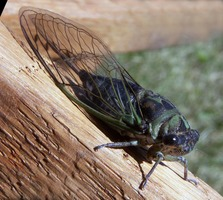
\includegraphics[width=0.8\linewidth]{cicada.jpg}
\caption{Une cigale}
\end{figure}

%----------------------------------------------------------------------------------------

\begin{table}[]
\begin{tabular}{lcccccc}
&BW&WL&WW&BL&G&Species\\\hline
\textbf{0}&0.25&28&11&28&0&0\\
\textbf{1}&0.16&26&11&22&1&0\\
\textbf{2}&0.26&31&11&27&0&2\\
\textbf{3}&0.16&26&9&21&1&0\\
\textbf{4}&0.26&30&12&26&0&0
\end{tabular}
\end{table}

\end{column} % End of the first column

\begin{column}{\sepwid}\end{column} % Empty spacer column

\begin{column}{\twocolwid} % Begin a column which is two columns wide (column 2)

\begin{columns}[t,totalwidth=\twocolwid] % Split up the two columns wide column

\begin{column}{\onecolwid}\vspace{-.6in} % The first column within column 2 (column 2.1)

%----------------------------------------------------------------------------------------
%	Variables
%----------------------------------------------------------------------------------------

\begin{block}{Variables de régression}

Aprés l'importation des données avec SageMath, on peut utiliser la commande

\texttt{pandas.plotting.scatter\_matrix}

pour visualizer toutes les graphes résultantes des les différents combinaisons possibles des variables.

\vspace*{1em}
On trouve que la graphe \textbf{(BW, WL)} resemble le mieux une droite, avec une coefficient de determination qui vaut $\simeq 0.32054$
\vspace*{1em}

\textbf{X} = BW = Poids\\
\textbf{Y} = WL = Longueur des ailes

\end{block}

%----------------------------------------------------------------------------------------

\end{column} % End of column 2.1

\begin{column}{\onecolwid}\vspace{-.6in} % The second column within column 2 (column 2.2)

%----------------------------------------------------------------------------------------
%	Statistiques descriptives
%----------------------------------------------------------------------------------------

\begin{block}{Statistique descriptive}

\begin{table}[]
\begin{tabular}{l|c|c}
&\ BW\ &\ WL\ \\\hline
Moy&0.179904&28.384615\\\hline
Médian&0.17&29\\\hline
Ecart-type&0.059259&2.261144\\\hline
Min&0.08&22\\\hline
Max&0.39&35\\
\end{tabular}
\end{table}

\end{block}

%----------------------------------------------------------------------------------------

\end{column} % End of column 2.2

\end{columns} % End of the split of column 2 - any content after this will now take up 2 columns width

%----------------------------------------------------------------------------------------
%	IMPORTANT RESULT
%----------------------------------------------------------------------------------------

%\begin{alertblock}{Important Result}
\vspace*{1em}
%Lorem ipsum dolor \textbf{sit amet}, consectetur adipiscing elit. Sed commodo molestie porta. Sed ultrices scelerisque sapien ac commodo. Donec ut volutpat elit.

%\end{alertblock} 

%----------------------------------------------------------------------------------------

\begin{columns}[t,totalwidth=\twocolwid] % Split up the two columns wide column again

\begin{column}{\onecolwid} % The first column within column 2 (column 2.1)

%----------------------------------------------------------------------------------------
%	Régression Linéaire
%----------------------------------------------------------------------------------------

\begin{block}{Régression Linéaire}

On obtient la courbe suivante:

\vspace*{75px}

%------------------------------------------------

\begin{figure}
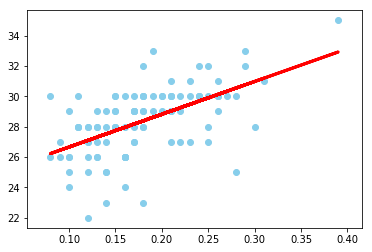
\includegraphics[width=0.8\linewidth]{figure.png}
\caption{Courbe de la régression linéaire}
\end{figure}

%----------------------------------------------------------------------------------------

\vspace*{1em}

\texttt{plt.scatter(X, Y, color="skyblue")\\
plt.plot(X, reg.predict(X), color="red", linewidth=3)}

\end{block}

%----------------------------------------------------------------------------------------

\end{column} % End of column 2.1

\begin{column}{\onecolwid} % The second column within column 2 (column 2.2)

%----------------------------------------------------------------------------------------
%	Résultats
%----------------------------------------------------------------------------------------

\begin{block}{Résultats}

%\begin{figure}
%\includegraphics[width=0.8\linewidth]{placeholder.jpg}
%\caption{Figure caption}
%\end{figure}

On trouve que:

\begin{align*}
    Y = a * X + b\\\\
    \text{avec:}\\
    \begin{cases}
        a &\simeq21.60317093 \\
        b &\simeq24.49812184 
    \end{cases}
\end{align*}

\vspace*{1em}
Quelques estimations:
\vspace*{1em}

\begin{table}[]
\begin{tabular}{c|c}
X\_test&Y\_predic\\\hline
0.35&32.05923167\\\hline
0.4&33.13939022\\\hline
0.45&34.21954876
\end{tabular}
\end{table}

\end{block}

%----------------------------------------------------------------------------------------

\end{column} % End of column 2.2

\end{columns} % End of the split of column 2

\end{column} % End of the second column

\begin{column}{\sepwid}\end{column} % Empty spacer column

\begin{column}{\onecolwid} % The third column

%----------------------------------------------------------------------------------------
%	CONCLUSION
%----------------------------------------------------------------------------------------

\begin{block}{Conclusion}

En conçlu bien qu'on peut appliquer la technique de régression linéaire sur le modèle constitué par le poids et le longueur des ailes d'une cigale, 
c'est qui peut aidez les chercheurs scientifiques dans la future. 

\vspace*{2em}

\end{block}

%----------------------------------------------------------------------------------------
%	REFERENCES
%----------------------------------------------------------------------------------------

\begin{block}{Références}

\nocite{*} % Insert publications even if they are not cited in the poster
\small{\bibliographystyle{unsrt}
\bibliography{sample}\vspace{0.75in}}

\vspace*{2em}

\end{block}

\begin{block}{Les bibliothéques Python}

\begin{center}
\begin{minipage}{0.14\textwidth}
\begin{itemize}
    \item \texttt{numpy}
    \item \texttt{matplotlib}
    \item \texttt{pandas}
    \item \texttt{scikit-learn}
\end{itemize}
\end{minipage}
\end{center}

\end{block}

%----------------------------------------------------------------------------------------

\end{column} % End of the third column

\end{columns} % End of all the columns in the poster

\end{frame} % End of the enclosing frame

\end{document}
